\textbf{{1. 链栈的定义}}

\textbf{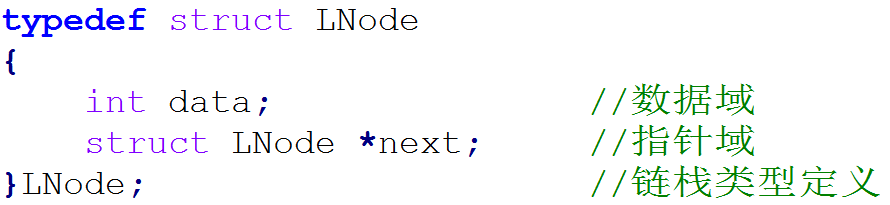
\includegraphics[width=2.81250in,height=0.64583in]{png-jpeg-pics/E67CB7E9F1DDEE7B7F76081BFC0A855F.png}\\
}

\textbf{{2. 链栈的基本操作}}

(1)入栈

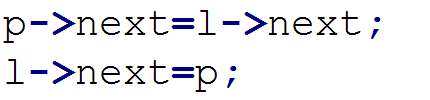
\includegraphics[width=1.35417in,height=0.31250in]{png-jpeg-pics/B40903111C8985FC06233A7AEA099426.png}

(2)出栈

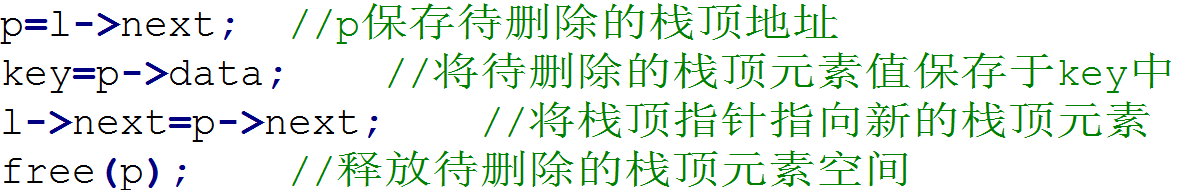
\includegraphics[width=3.43750in,height=0.55208in]{png-jpeg-pics/7FDDA5961F623A82F98AD8A1A54D51D5.png}
